\documentclass[main.tex]{subfiles}
\begin{document}
\section{神奇bug在哪里}
本人编写代码耗时5天,调试耗时6天,时间甚短,除在调试过程中已暴露出的bug,还应有许多bug待测试。现将已遇到的问题及解决方法罗列如下,望观者引以为戒。\\

\textbf{2024/1/29}
\begin{enumerate}
    \item 现象:adc.series\_ecd数据解算溢出
    \item 原因:adc.rounds\_cnt定义为uint32类型,在反转时溢出
    \item 解决:修改adc.rounds\_cnt类型为int32类型 \\
\end{enumerate}

\begin{enumerate}
    \item 现象:程序跑飞,运行到未执行到的函数,中断进入一次后不再进入
    \item 原因:任务执行部分形参为FOC\_Typedef\_t *foc,在清除时写成\&foc
    \item 解决:删去\&
\end{enumerate}
\rule{\linewidth}{0.3pt}

\textbf{2024/1/30}
\begin{enumerate}
    \item 现象:
    \begin{lstlisting}[language=C]
    //会导致代码进入hard_fault()
    foc->cos_theta = arm_cos_f32(encoder_elec_temp)
    foc->sin_theta = arm_sin_f32(encoder_elec_temp)
    foc->elec_angle = Elec_Angle_Get();
    foc->Curr.Ia = Ia_Get();
    foc->Curr.Ib = Ib_Get();
    
    //代码不会进入hard_fault()
    test1 = arm_cos_f32(encoder_elec_temp);
    test2 = arm_sin_f32(encoder_elec_temp);
    
    //代码不会进入hard_fault()
    foc->cos_theta = 1.0f;
    foc->sin_theta = 0.0f;
    \end{lstlisting}
    \item 原因:void FOC\_Task(FOC\_Typedef\_t *foc)调用时没有写参数
    \item 解决:调用函数改为FOC\_Task(\&foc);\\
\end{enumerate}

\begin{enumerate}
    \item 现象:foc$\rightarrow$elec\_angle, foc$\rightarrow$sin\_theta 和 foc$\rightarrow$cos\_theta反馈不正确
    \item 原因:未知
    \item 解决:使用foc->elec\_angle进行计算,而不是adc.elec\_angle \\
\end{enumerate}

\begin{enumerate}
    \item 现象:电机霍尔传感器呈阶梯状
    \item 原因:TIM7为20kHz定时器中断,在定时器中断中获取ADC的值,但ADC中断触发频率远低于20kHz, 1s内仅能触发300次左右,具体原因可能是DMA中断比ADC中断优先级高,ADC中断执行完跳转到DMA中断,没有触发ADC中断回调,仅在少数时间跳转到ADC中断函数中,导致了消息解算速度很慢,信号呈阶梯状
    \item 解决:ADC中断关闭,将信号处理放在TIM7定时器中断中, 判断ADC信号解算完成之后执行FOC \\
\end{enumerate}

\begin{enumerate}
    \item 现象:pid初始化后kp, ki, kd参数依旧为0
    \item 原因:参数在main函数初始化,初始状态处在未使能时会进行PID\_Clear操作,又把PID三个参数清0
    \item 解决:定义一个flag位,当电机失能时flag位置为0,使能时若flag位为0,则进行PID初始化,并将flag位置为1 \\
\end{enumerate}

\begin{enumerate}
    \item 现象:速度环、位置环、混合模式下依旧不能成功初始化kp, ki, kd
    \item 原因:定义kp, ki, kd三个参数时定义错误,写成了
    \begin{lstlisting}[language=C]
        const Motor_Mix_PID[3] = {1.1f, 2.2f, 3.3f};
    \end{lstlisting}
    \item 解决:加上数据类型fp32(好愚蠢>︿<)
    \begin{lstlisting}[language=C]
        const fp32 Motor_Mix_PID[3] = {1.1f, 2.2f, 3.3f};
    \end{lstlisting}
\end{enumerate}
\rule{\linewidth}{0.3pt}
\textbf{2024/1/31}

\begin{enumerate}
    \item 现象:电机无法做到速度闭环,反转时出现卡顿现象,且方向与设定方向相反
    \item 原因:纯电压控制时也出现卡顿现象,若将电角度自定义为累加,卡顿现象变明显
    \item 解决:修改void SVPWM\_Calc(FOC\_Typedef\_t *foc)函数,改变切换时间点的计算,修改后和前述SVPWM算法一致\\
\end{enumerate}

\begin{enumerate}
    \item 现象:互为相反数的电压设置,电机正转和反转速度不一样,马鞍波波形均为标准马鞍波,但频率不同
    \item 原因:未校准零位,正反转效率可能不同
    \item 解决:校准完零位后,正反转速度差距更大\\
\end{enumerate}

\begin{enumerate}
    \item 现象:ADC采样电流数据在jscope中溢出,在watch窗口中正常
    \item 原因:示波器bug
    \item 解决:无需解决\\
\end{enumerate}

\begin{enumerate}
    \item 现象:给定电压电机不转,将零位设为0后恢复;速度闭环只有一个方向能闭
    \item 解决:下班时间,先溜为妙,玄学问题,明日再看,今天是失败的一天
\end{enumerate}
\rule{\linewidth}{0.3pt}

\textbf{2024/2/1}
\begin{enumerate}
    \item 现象:TIM7中断触发频率很低,10s内仅能触发67000余次,但配置无误
    \item 原因:在数据解算时使用了双层for循环嵌套,阻塞了时钟中断
    \item 解决:删除其中一层循环次数多的循环嵌套,改写为多个值相加。解决了\textbf{2024/1/31}产生的所有问题。\\
\end{enumerate}

\begin{enumerate}
    \item 现象:速度目标设置过高时无法达到目标设定值
    \item 原因:被Vd、Vq约束所限制
    \item 解决:设定Iq最大输出为母线电压的2/3, 取消Vq限制
\end{enumerate}
\rule{\linewidth}{0.3pt}

\textbf{2024/2/20}
\begin{enumerate}
    \item 现象:目标速度设为0时经过pid计算电机还是以极高的速度运行,这种现象在参数写入flash后消失
    \item 原因:电机校准问题
    \item 解决:不应每次上电都校准,每个电机校准一次,将零点写入,后续读取零点即可
\end{enumerate}
\rule{\linewidth}{0.3pt}

\textbf{2024/2/21}
\begin{enumerate}
    \item 现象:can通信后解算出的目标速度与接收端的RxBuffer不一致
    \item 原因:未知
    \item 解决:使用union进行int和float的转换,而非强制转换
    \begin{lstlisting}[language=C]
        temp_union1.int32_ = (RxBuffer[3] << 24)|(RxBuffer[4] << 16)|
                             (RxBuffer[5] << 8)|(RxBuffer[6]);
                             
        goal_set.speed_set = temp_union1.fp32_;
    \end{lstlisting}
\end{enumerate}

\begin{enumerate}
    \item 现象:调试状态正常使用,断电后重新上电不能工作
    \item 原因:未知
    \item 解决:修改后面问题后本问题突然迎刃而解\\
\end{enumerate}

\begin{enumerate}
    \item 现象:yaw轴电机有时会飘,没有收到速度为0命令
    \item 原因:受到pitch轴信息影响,pitch轴电机代码仍为原代码
    \item 解决:删除pitch轴发送信息,两套为完全不同的协议,互串
\end{enumerate}
\rule{\linewidth}{0.3pt}

\textbf{2024/2/27}
\begin{enumerate}
    \item 现象:pitch轴电机所需力矩过大时,速度环发散
    \begin{figure}[H]
        \centering
        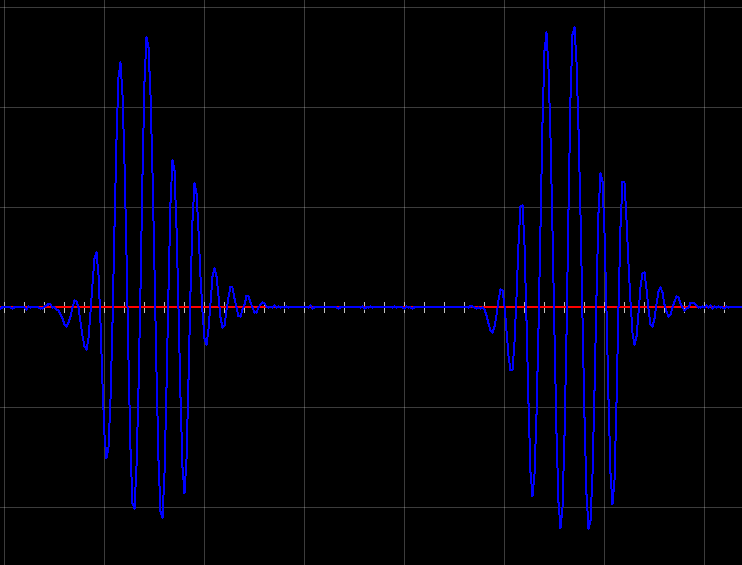
\includegraphics[width=0.4\textwidth]{img/img_1.4.1.png}
        \caption{速度目标为0:发散}
        \label{goal-0}
    \end{figure}
    \begin{figure}[H]
        \centering
        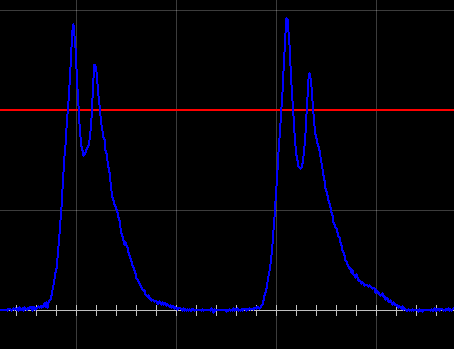
\includegraphics[width=0.4\textwidth]{img/img_1.4.2.png}
        \caption{速度目标为100:震荡}
        \label{goal-100}
    \end{figure}
    \item 原因:零位校准问题
    \item 解决:手动校准:固定电压输出,获得最大速度的电角度偏移值即为零位\\
\end{enumerate}

\begin{enumerate}
    \item 现象:速度为+100和-100时电流相差很远且二者效果不同,速度为+100时电流更大,但速度波动小

          电压互为相反数时实际电流一样;电流互为相反数时实际电流相差更大。

          经过校准后在某些零位值时,速度目标为0rpm电机依旧旋转
    \begin{figure}[H]
        \centering
        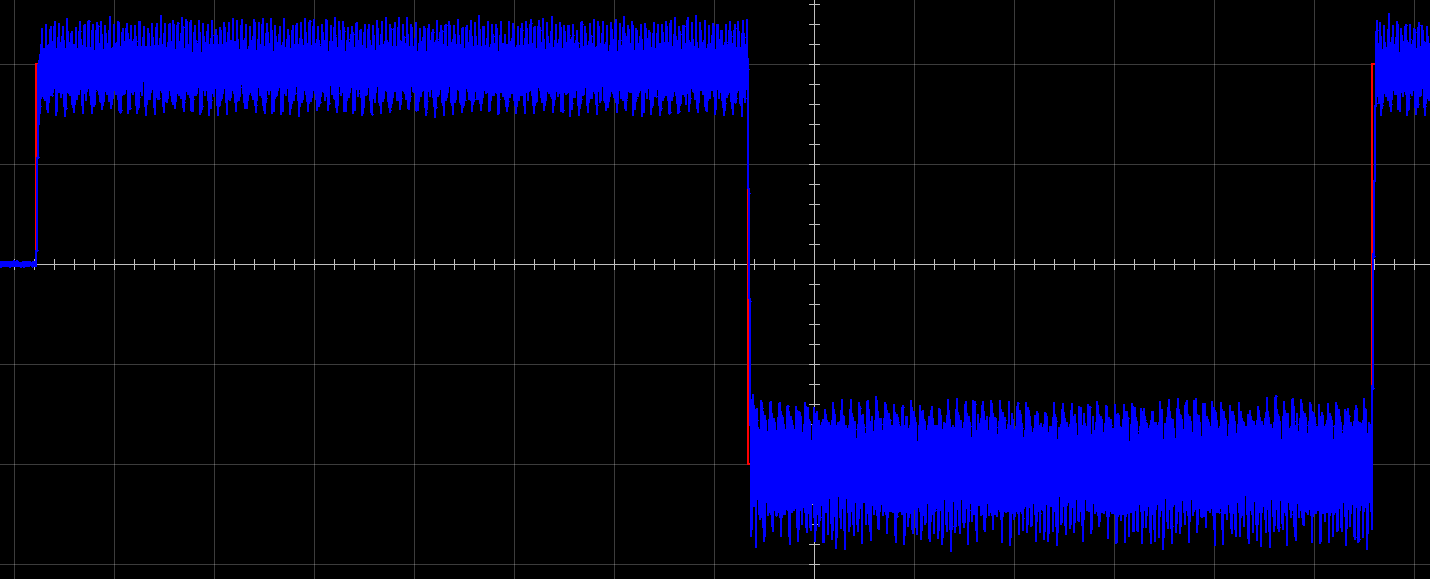
\includegraphics[width=0.6\textwidth]{img/img_1.4.3.png}
        \caption{不同速度目标的反馈效果}
        \label{speed equal to 100 and -100}
    \end{figure}
    \item 原因:由于未知原因导致q轴和d轴相反,导致速度目标为0时,受到微小扰动导致给定的q轴电流使电机依旧旋转
    \item 解决:手动校准\\
\end{enumerate}

\begin{enumerate}
    \item 现象:速度拨动大且有超调
    \begin{figure}[H]
        \centering
        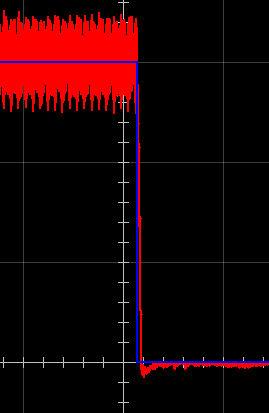
\includegraphics[width=0.3\textwidth]{img/img_1.4.4.png}
        \caption{300rpm时的超调现象}
        \label{PID params is not correct}
    \end{figure}
    \item 原因:kp参数过大
    \item 解决:调小速度环和电流环的kp
\end{enumerate}

\end{document}

